\chapter{Fusione tramite deep learning}

\section{Le componenti della CNN}
\subsection{Reti neurali residuali}
Le reti neurali residuali, o ResNet, sono stati introdotti da Microsoft nel 2015 battendo il record della competizione ILSVRC con un errore del 3.6\% \cite{resnet}, superando per la prima volta le prestazioni umane.\\
L'idea che sta alla base delle reti neurali residuali è l'utilizzo di un particolare tipo di blocco, il \textit{residual block}, che sfrutta il concetto delle \textit{skip connection}. \\
Vediamo ora il modello del residual block:
\begin{figure}[ht]
    \centering
    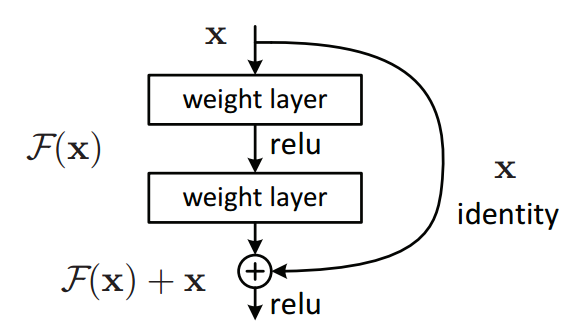
\includegraphics[width=0.5\columnwidth]{res_block.png}
    \caption[Residual block]{Schema del residual block}
\end{figure}\\
Ogni blocco consiste in una serie di strati, ottenendo una certa $F(x)$, seguito da una \textit{skip connection} che aggiunge al risultato l'input del blocco stesso. Dunque in uscita dal blocco si ha
$$ H(x)=F(x)+x $$
Attraverso la concatenazione di blocchi di questo tipo, ResNet impara a predire l'output non attraverso l'apprendimento di una trasformazione diretta dei dati di input, ma attraverso l'apprendimento del termine $F(x)$, detto \textit{residuo}, da sommare al dato di input per arrivare all'output. Tale modello semplifica la costruzione di strati di identità, basta infatti spingere $F(x)$ verso zero e lasciare l'output come x. Ciò permette agli strati più profondi della rete di alterare poco i concetti già appresi dagli strati precedenti, preservando così le informazioni. Questa architettura ha permesso di creare reti molto più profonde, fino a 152 strati.

\subsection{Batch Normalization}
Durante il processo di addestramento, gli esempi del training set vengono processati in gruppi, detti mini-batch, di dimensione fissa per velocizzare la fase di train sfruttando il parallelismo offerto dalle GPU. La \textit{Batch Normalization} è una tecnica che consiste nel normalizzare i dati del mini-batch ad ogni strato intermedio della rete. In questo modo si riduce il così detto \textit{Internal Covariance Shift}. L'utilizzo del batch normalization ha l'intento di velocizzare il training della rete neurale e migliorarne la stabilità e le performance. Questa operazione si è rivelata particolarmente efficace nelle reti neurali residuali.

\subsection{Bottleneck}
Il modello ResNet introduce il così detto design a "collo di bottiglia". L'idea che sta dietro all'utilizzo di questo design è quello di ridurre le dimensioni dell'input del blocco residuale prima di effettuare la convoluzione 3x3.
\begin{figure}[ht]
    \centering
    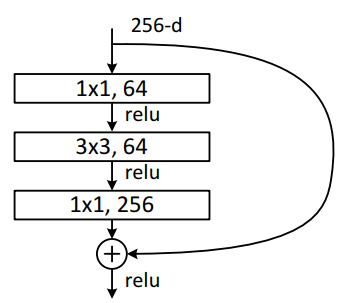
\includegraphics[width=0.4\columnwidth]{bottleneck.png}
    \caption[Bottleneck]{Il design a collo di bottiglia utilizzato dal  ResNet}
\end{figure}
La riduzione della dimensionalità viene eseguita con uno strato di convoluzione 1x1, lasciando lo strato di convoluzione 3x3 con delle dimensioni di input/output più ridotte, tenendo così un numero di parametri molto più ristretto. Infine, l'ultimo strato 1x1 ha lo scopo di ripristinare le dimensioni a quelle iniziali. Questo permette un tempo di addestramento più veloce, senza pesare sulle prestazioni \cite{resnet}.

\subsection{Convoluzione dilatata}
Il vantaggio della convoluzione dilatata è la possibilità di catturare più indizi dall'input, espandendo il campo recettivo di una convoluzione 2D.
\begin{figure}[ht]
    \centering
    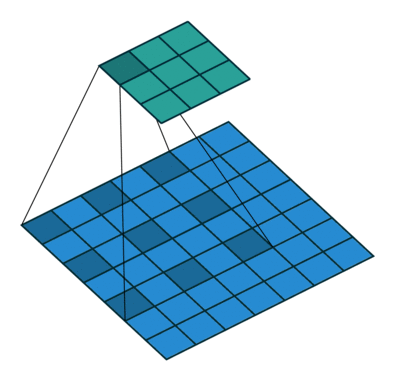
\includegraphics[width=0.5\columnwidth]{dilated_convolution.png}
    \caption[Convoluzione dilatata]{Illustrazione della convoluzione dilatata}
\end{figure}\\
In realtà, anche utilizzando un filtro di dimensioni maggiori si ha un receptive field allargato, ad esempio una convoluzione 3x3 dilatata con rate $r=2$ ha lo stesso campo recettivo di una normale convoluzione 5x5. Tuttavia, il numero di parametri del modello con dilatazione può essere notevolmente ridotto. Un kernel $k\times k$ mantiene, infatti, $k\times k$ parametri avendo però un campo recettivo pari a $k_e\times k_e$ con $k_e=k+(k-1)(r-1)$.

\section{la rete neurale selezionata}
L'architettura della rete neurale convoluzionale utilizzata in questo lavoro di tesi è formato da una rete neurale residuale con bottleneck, batch normalization e convoluzione dilatata. Il blocco residuale utilizzato è il seguente:
\begin{figure}[ht]
    \centering
    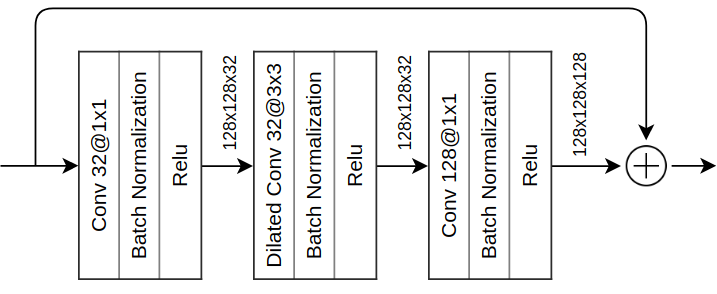
\includegraphics[width=0.6\columnwidth]{my_res_block.png}
    \caption[Diagramma del blocco residuale]{Diagramma del blocco residuale}
\end{figure}\\
La CNN differisce dalla ResNet per l'assenza dello strato finale \textit{fully connected}, si tratta quindi di una rete \textit{fully convolutional} che ha come output una singola feature map con la stessa risoluzione delle immagini in input. L'architettura selezionata è una concatenazione di sei blocchi residuali, seguito da una convoluzione che combina le 128 feature map restituendo l'immagine risultante.
\begin{figure}[ht]
    \centering
    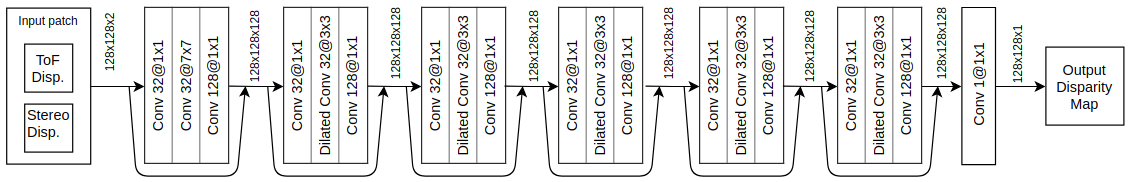
\includegraphics[width=1\columnwidth]{net_scheme.png}
    \caption[Architettura della CNN]{Diagramma della CNN. Per sintesi non ho incluso gli strati di normalizzazione e rettificazione lineare.}
\end{figure}

\section{Il processo di training}
\subsection{Loss function e ottimizzazione}
\paragraph{Loss function} Per poter minimizzare l'errore di output della rete neurale è necessario definire tale errore.\\
Le due funzioni di loss valutate in questo lavoro sono le norme l1 e l2, detti anche \textit{mean absolute error} e \textit{mean squared error}.
$$MAE=\frac{1}{n} \sum_{j=1}^{n} |y_j-\hat{y_j}|$$
$$MSE=\frac{1}{n} \sum_{j=1}^{n} (y_j-\hat{y_j})^2$$
Da un veloce confronto, le due norme danno risultati sperimentali simili. È stato deciso di utilizzare la norma l2, una delle loss function maggiormente utilizzate.

\paragraph{Ottimizzazione} Il training è stato effettuato con algoritmo di ottimizzazione \textit{Adam}. Questo metodo di ottimizzazione è una estensione della discesa stocastica del gradiente che ha visto un largo utilizzo in molte applicazioni del deep learning nella computer vision e nell'elaborazione del linguaggio naturale. Il nome \textit{Adam} deriva da \textit{adaptive moment estimation}. Questo metodo combina i vantaggi di AdaGrad e RMSProp, modificando i parametri di learning rate in modo adattivo in base alle stime dei momenti di primo e secondo ordine dei gradienti. Il learning rate scelto è $lr=0.001$ mentre i fattori di decadimento impostati sono $\beta_1=0.9$ e $\beta_2=0.999$

\subsection{Inizializzazione delle variabili}
L'inizializzazione dei pesi della rete neurale è una delicata operazione che se non effettuata bene potrebbe impedire la convergenza della rete durante l'apprendimento. Infatti, se i pesi vengono inizializzati troppo piccoli allora andando in profondità nella rete il segnale comincia ad attenuarsi, fino a diventare inutilizzabile. D'altra parte, se i pesi sono troppo grandi allora il segnale in ingresso si amplifica fino a saturare i neuroni. Impostare i pesi a zero ha poco senso in quanto renderebbe la rete equivalente a un modello lineare. Perciò la soluzione è inizializzare i pesi attraverso generazioni casuali secondo una certa distribuzione adeguata.\\
La distribuzione utilizzata in questo lavoro è quello proposto da Xavier \cite{xavier}. L'idea è quella di utilizzare una distribuzione gaussiana con media nulla e una certa varianza finita. Consideriamo un neurone lineare:
$$y = w_1 x_1 + w_2 x_2 + ... + w_N x_N + b$$
Mano a mano che si processano i vari strati, vogliamo che la varianza rimanga la stessa. Questo aiuta ad evitare che il segnale esploda oppure che si attenui verso lo zero. In altre parole vogliamo inizializzare i pesi in modo che la varianza rimanga uguale per $x$ e $y$.\\
Calcoliamo ora la varianza di $y$:
$$Var(y) = Var(w_1x_1 + w_2x_2 + ... + w_Nx_N + b)$$
Assumiamo che le variabili $x_i$ siano indipendenti e calcoliamo le varianze dei termini all'interno delle parentesi di destra. Abbiamo:
$$Var(w_ix_i) = E(x_i)^2Var(w_i) + E(w_i)^2Var(x_i) + Var(w_i)Var(x_i)$$
Abbiamo assunto che gli input e i pesi abbiano media nulla, perciò abbiamo:
$$Var(w_ix_i) = Var(w_i)Var(x_i)$$
Notiamo che $b$ è costante perciò sparisce. Sostituiamo nell'equazione iniziale:
$$Var(y) = Var(w_1)Var(x_1) + ... + Var(w_N)Var(x_N)$$
Dato che sono identicamente distribuiti, possiamo scrivere:
$$Var(y) = N * Var(w_i) * Var(x_i)$$
Perciò, se vogliamo che la varianza di y sia uguale alla varianza di x, allora il termine $N*Var(w_i)$ deve valere 1. Dunque:
$$N * Var(wi) = 1$$
$$Var(w_i) = \frac{1}{N}$$
Abbiamo trovato la formula di \textbf{inizializzazione di Xavier}, non dobbiamo fare altro che inizializzare i pesi secondo una normale a media nulla e varianza pari all'inverso del numero di connessioni in ingresso.

\subsection{Iperparametri}
batch size e learning rate
\subsection{Early stopping}
